\documentclass[a4paper,12pt]{book}
\usepackage[utf8]{inputenc}

\usepackage{rachwidgets}


\newcommand{\laClass}       {CS 211}
\newcommand{\laSemester}    {Spring 2018}
\newcommand{\laChapter}     {6.6}
\newcommand{\laType}        {Exercise}
\newcommand{\laPoints}      {5}
\newcommand{\laTitle}       {Matrices and Markov Chains}
\newcommand{\laDate}        {Mar 6, 2018}
\setcounter{chapter}{5}
\setcounter{section}{1}
\addtocounter{section}{-1}
\newcounter{question}

\toggletrue{answerkey}
\togglefalse{answerkey}


\title{}
\author{Rachel Singh}
\date{\today}

\pagestyle{fancy}
\fancyhf{}

\lhead{\laClass, \laSemester, \laDate}

\chead{}

\rhead{\laChapter\ \laType\ \iftoggle{answerkey}{ KEY }{}}

\rfoot{\thepage\ of \pageref{LastPage}}

\lfoot{\scriptsize By Rachel Singh, last updated \today}

\renewcommand{\headrulewidth}{2pt}
\renewcommand{\footrulewidth}{1pt}

\begin{document}




\footnotesize
~\\ 
\textbf{\laChapter\ \laType: } In-class exercises are meant to introduce you to a new topic
and provide some practice with the new topic. Work in a team of up to 4 people to complete this exercise.
You can work simultaneously on the problems, or work separate and then check your answers with each other.
Completion score is given for this assignment.

~\\
Team:\\
(1) \tab[6cm] (2) \\
(3) \tab[6cm] (4)

\hrulefill
\normalsize 


\notonkey{
% ASSIGNMENT ------------------------------------ %

    \section{\laTitle}

    \subsection{The Gambler's Ruin Problem}
        \begin{intro}{\ }
            \footnotesize
            \textbf{The Gambler's Ruin Problem} \\
            Page 478 of the book highlights a game played between
            two characters: Player ``H" and Player ``T". Each character begins with
            a certain amount of markers (or tokens), and they play
            by flipping a \textbf{coin}. Whenever one
            of them loses a ``round", they give one marker to their opponent.

            \begin{center}
                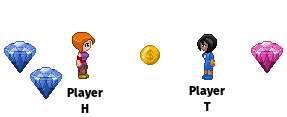
\includegraphics{images/6-6-game.png}
            \end{center}

            If a \textit{heads} is flipped, then Player H wins a marker from Player T.
            For a \textit{tails}, Player T wins a marker from Player H.
            The game is over once somebody is out of markers.

            \paragraph{Game setup:} For the game we'll be talking about
            in thie example, the rules are:

            \begin{itemize}
                \item   There are 3 total markers (so one player will have
                more markers than the other)

                \item   Once somebody is out of markers, the game is over.

                \item   Each coin flip, the loser gives one of their markers
                to the other player. (One gains, one loses)
            \end{itemize}
            
            \paragraph{Game states:} Before we start modeling the game
            with a matrix, let's map out all the game states.
            We won't worry about what is the
            beginning state, and each coin flip, one person gains a marker
            and one person loses a marker. There are four possible states
             in the game:

             \begin{center}
                 \begin{tabular}{c c c}
                     State \# & H's markers & T's markers \\ \hline
                     1 & 0 & 3 \\
                     2 & 1 & 2 \\
                     3 & 2 & 1 \\
                     4 & 3 & 0
                 \end{tabular}
             \end{center}

            \paragraph{State diagram:}  Given these states,
            and the fact that each coin flip one person loses a marker
            and gives it to the other, our state diagram
            would look like:
            
            \begin{center}
                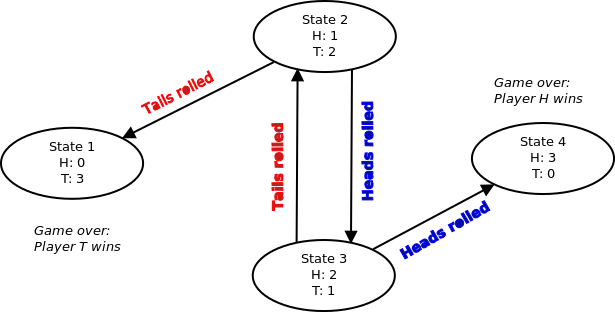
\includegraphics[width=10cm]{images/6-6-states.png}
            \end{center}

            \paragraph{State change matrix:} Now we will build out
            a matrix to show the probability of switching between states.

            The matrix will be $4 \times 4$. Each \textbf{row} will be
            a state, and each cell in that row is the probability of going
            from that state to a new state.

            \begin{center}
                \begin{tabular}{l c c c c}
                    & State 1 & State 2 & State 3 & State 4
                    \\
                    State 1 $\to$ &
                        1 & 0 & 0 & 0
                    \\
                    State 2 $\to$ &
                        1/2 & 0 & 1/2 & 0
                    \\
                    State 3 $\to$ &
                        0 & 1/2 & 0 & 1/2
                    \\
                    State 4 $\to$ &
                        0 & 0 & 0 & 1
                \end{tabular}
            \end{center}

            This matrix is in the format, ``from $row$ state to $col$ state".
            In Row 2, the probability of going from (State 2 $\to$ State 1) is 1/2,
            because the coin flip has a half chance of being heads, and a half chance
            of being tails.

            State 1 and State 4 they are gameover states: you cannot
            move from State 1 to another state, so it has a 1 in that cell.
            
        \end{intro}

    \newpage

    \stepcounter{question}
    \begin{questionNOGRADE}{\thequestion}
        Let's say a game starts where Player H has 2 markers and
        player 1 has 1 marker. This is state 3.

        \begin{center}
            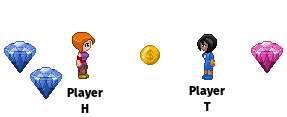
\includegraphics{images/6-6-game.png}
        \end{center}

        What is the probability of...

        \begin{itemize}
            \item[a.] Going from State 3 to State 1? ~\\ \vspace{2cm}
            \item[b.] Going from State 3 to State 2? ~\\ \vspace{2cm}
            \item[c.] Going from State 3 to State 3? ~\\ \vspace{2cm}
            \item[d.] Going from State 3 to State 4? ~\\ \vspace{2cm}
                \solution{1/2}{}
        \end{itemize}
    \end{questionNOGRADE}

    \newpage
    
        \begin{intro}{Transition Matrix}
            If you have a game with states 1 through $n$, then your
            transition matrix $M$ is

            $M_{i,j} = Prob($the game changes from state $i$ to state $j$ in one move$)$.
            \footnote{Discrete Structures, Ensley and Crawley}
        \end{intro}

        \stepcounter{question}
        \begin{questionNOGRADE}{\thequestion}
            Let's say in the game there are 2 total markers instead of three.

            \begin{enumerate}
                \item[a.]   What are all the states in the game? ~\\ \vspace{2cm}
                \item[b.]   Draw the transition matrix for this game.
            \end{enumerate}
        \end{questionNOGRADE}

    \newpage 


        \begin{intro}{Transition Matrix}
            Given the matrices $M$ and $N$, where the amount of \textit{rows} in $M$
            is the same amount of \textit{columns} in $N$,
            we can find the product $P = M \cdot N$ where each entry at
            row $i$, column $j$ of $P$ is the row-column product of
            row $i$ from $M$ and column $j$ from $N$. In other words,
            \footnote{Discrete Structures, Ensley and Crawley}

            $$ P_{i,j} = M_{i,1} \cdot N_{1,j} + M_{i,2} \cdot N_{2,j} + ... $$
        \end{intro}


    \stepcounter{question}
    \begin{questionNOGRADE}{\thequestion}
        Calculate the product $M \cdot M$ (aka $M^{2}$) for our
        original game with 3 markers.
        
        \begin{center}
            \large
            \begin{tabular}{ l | c c c c |}
                & Col 1 & Col 2 & Col 3 & Col 4
                \\ \hline
                Row 1 & 1 & 0 & 0 & 0
                \\
                Row 2 & 1/2 & 0 & 1/2 & 0
                \\
                Row 3 & 0 & 1/2 & 0 & 1/2
                \\
                Row 4 & 0 & 0 & 0 & 1
            \end{tabular}
        \end{center}
        
        The result ends up being the probability that the game processes from
        state $i$ to state $j$ in \textbf{two} moves.
        
            asdfasjdlifjasdlkfjalksdjf
    \end{questionNOGRADE}

        
}{
% KEY ------------------------------------ %

    \begin{enumerate}
        \item   
            \begin{itemize}
                \item[a.] Going from State 3 to State 1? \tab 0
                \item[b.] Going from State 3 to State 2? \tab 1/2
                \item[c.] Going from State 3 to State 3? \tab 0
                \item[d.] Going from State 3 to State 4? \tab 1/2
            \end{itemize}

        \item
            \begin{itemize}
                \item[a.]   
                    1. H: 0, T: 2   \tab
                    2. H: 1, T: 1   \tab
                    3. H: 2, H: 0
                \item[b.]   
                    \begin{tabular}{l c c c}
                        & State 1 & State 2 & State 3
                        \\
                        State 1 $\to$ &
                            1 & 0 & 0 
                        \\
                        State 2 $\to$ &
                            1/2 & 0 & 1/2
                        \\
                        State 3 $\to$ &
                            0 & 0 & 1
                    \end{tabular}
            \end{itemize}

        \item   
            \begin{tabular}{| c c c c |}
                1 & 0 & 0 & 0
                \\
                1/2 & 1/4 & 0 & 1/4
                \\
                1/4 & 0 & 1/4 & 1/2
                \\
                0 & 0 & 0 & 1
            \end{tabular}
    \end{enumerate}

}



\end{document}

